\subsection{Descriptive Statistics and Stylized Facts}
\label{sec:descriptive}

Descriptive statistics confirmed that all three canonical stylized facts were present in both the in-sample (2014--2024, $T = 2{,}766$) and out-of-sample (2025, $T = 219$) windows (Table~\ref{tab:descriptive}).
The in-sample excess growth rates exhibited excess kurtosis of 7.707, strong negative skewness ($-0.753$), and a Jarque--Bera statistic of 7107.4, decisively rejecting the null hypothesis of normality ($p < 0.001$).
The Ljung--Box test on absolute returns rejected the null of no autocorrelation ($\text{LB} = 3057.9$, $p < 0.001$), confirming pronounced volatility clustering.
The Ljung--Box test on raw returns also rejected ($\text{LB} = 145.3$), reflecting mild serial dependence in the level series.

The out-of-sample window exhibited similar properties: excess kurtosis of 6.242, stronger negative skewness ($-1.071$), and a Jarque--Bera statistic of 397.4.
Notably, the Ljung--Box test on raw OoS returns failed to reject ($\text{LB} = 28.1$), consistent with efficient pricing in the shorter sample, while the test on absolute returns strongly rejected ($\text{LB} = 150.4$), confirming that volatility clustering persisted in the test period.
These properties are visualized in Figure~\ref{fig:stylized_facts}.

\begin{table}[t]
\centering
\caption{Descriptive statistics and stylized-fact tests for SPY daily excess growth rates. IS: 2014--2024 ($T = 2{,}766$); OoS: 2025 ($T = 219$). JB = Jarque--Bera normality test. LB = Ljung--Box autocorrelation test at lag~20. $^*$~denotes rejection at $\alpha = 0.05$.}
\label{tab:descriptive}
\begin{tabular}{lcc}
\toprule
Statistic & IS Observed & OoS Observed \\
\midrule
Mean (annualized) & 0.11 & 0.13 \\
Std Dev (annualized) & 2.14 & 2.31 \\
Skewness & $-0.753$ & $-1.071$ \\
Excess Kurtosis & 7.707 & 6.242 \\
JB test statistic & 7107.4 & 397.4 \\
JB decision & reject$^*$ ($p < 0.001$) & reject$^*$ ($p < 0.001$) \\
LB test on $G_t$ (lag 20) & reject$^*$ (145.3) & fail to reject (28.1) \\
LB test on $|G_t|$ (lag 20) & reject$^*$ (3057.9) & reject$^*$ (150.4) \\
\bottomrule
\end{tabular}
\end{table}

\begin{figure}[t]
\centering

\includegraphics[width=\textwidth]{sections/figs/Fig-1-Stylized-Facts.pdf}
\caption{Empirical stylized facts of SPY daily excess growth rates (2014--2024). Panel~(a): leptokurtic marginal distribution with Gaussian and Laplace fits. Panel~(b): normal Q-Q plot confirming heavy tails. Panel~(c): near-zero autocorrelation of raw returns. Panel~(d): persistent autocorrelation of absolute returns characterizing volatility clustering.}
\label{fig:stylized_facts}
\end{figure}

\subsection{Model Selection: Why $K = 18$}
\label{sec:model_selection}

We trained continuous Gaussian HMMs for $K \in \{3, 6, 9, 12, 15, 18, 21\}$ states on the SPY in-sample window using the Baum-Welch algorithm with $\texttt{max\_iter} = 60$ and quantile-based initialization, and evaluated every fitted model on (i) the four information criteria of equation~\eqref{eq:information_criteria}, following the HMM state-selection methodology of \citet{nguyen2018hidden}, and (ii) the full seven-metric distributional battery.
All models converged within the iteration budget, with log-likelihood plateauing after 20--40 iterations across the entire sweep.
The full sensitivity table is reproduced in Appendix~\ref{sec:supplemental} (Table~\ref{tab:sensitivity}); Figure~\ref{fig:k_sweep_summary} summarizes the distributional pass rates and ACF-MAE as a function of $K$.

Three patterns emerge.
First, the information-criterion surface flattens over the upper half of the sweep: AIC and HQC continue to improve mildly with $K$, while BIC and CAIC, which penalize the $K^2 + 2K - 1$ parameters more heavily, reach their joint minimum in the $K \in \{15, 18, 21\}$ region.
This narrows the sweep to a three-state-count band before any fidelity metric is consulted.
Second, distributional fidelity rises across the $K$ sweep and plateaus in the $K \in \{15, 18, 21\}$ band for CHMM-N: IS KS rises from 88.7\% ($K=3$) to 95.2\% ($K=18$) and 96.5\% ($K=21$), IS AD from 79.2\% to 88.3\% at $K=18$ (89.1\% at $K=21$), OoS KS from 92.8\% to 94.0\% at $K=18$, and OoS AD from 84.9\% to 88.7\% at $K=18$ (see Table~\ref{tab:sensitivity_multi}).
Third, ACF-MAE is remarkably stable across the sweep (0.045--0.051) and is actually lowest at $K=3$.
This establishes a mild \emph{distributional--temporal tradeoff}: higher $K$ buys distributional accuracy, lower $K$ buys marginally better ACF, and both are available within a narrow band.
$K = 18$ sits inside the IC-minimizing region and, together with $K \in \{15, 21\}$, attains the highest distributional pass rates in the sweep; it also achieves the largest simulated kurtosis (5.03) among CHMM-N fits in this band, closest to the observed 7.71.
We therefore report the remainder of Section~\ref{sec:results} at $K = 18$ and relegate the sensitivity panel to the appendix.

Figure~\ref{fig:model_internals} shows the fitted model internals for $K = 18$: the learned emission distributions span the full range of observed returns, with tail states capturing extreme crash and boom regimes.
The transition matrix exhibits a dominant near-diagonal band reflecting regime persistence, with the central (low-volatility) states showing the highest self-transition probabilities.
Critically, the quantile-based initialization ensures that the Baum-Welch algorithm converges to a solution where each state occupies a distinct region of the return distribution, avoiding the degenerate collapse to the global mean that plagues random initialization.

\begin{figure}[t]
\centering
\begin{subfigure}[b]{0.48\textwidth}
    
\includegraphics[width=\textwidth]{sections/figs/Fig-Emission-PDFs-K18.pdf}
    \caption{Emission distributions ($K = 18$)}
\end{subfigure}
\hfill
\begin{subfigure}[b]{0.48\textwidth}
    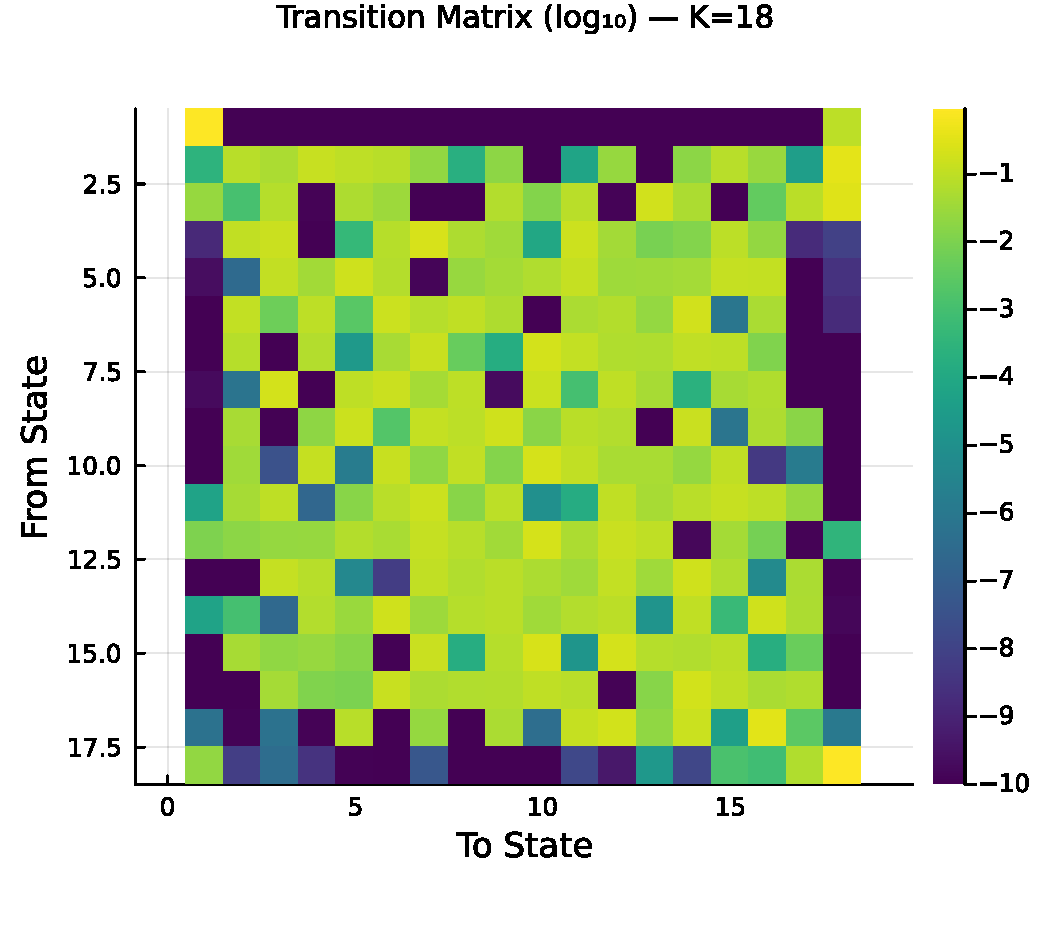
\includegraphics[width=\textwidth]{sections/figs/Fig-Transition-Matrix-K18.pdf}
    \caption{Transition matrix (log$_{10}$ scale)}
\end{subfigure}
\caption{Fitted model internals for SPY at the selected state resolution $K = 18$. (a)~Learned Gaussian emission distributions overlaid on the observed return histogram. (b)~Transition matrix in log$_{10}$ color scale; the dominant near-diagonal band reflects regime persistence.}
\label{fig:model_internals}
\end{figure}

\subsection{Seven-Model Comparison}
\label{sec:model_comparison}

Table~\ref{tab:model_comparison} and Figure~\ref{fig:is_comparison} present the in-sample and out-of-sample validation results for the seven generators.
The benchmark set was constructed to mimic the prior paper's evaluation exactly, adding the two discrete HMM variants of \citet{alswaidan2026hybrid} (NJ and WJ) to the original four baselines (Bootstrap, Gaussian, Laplace, GARCH(1,1)) and replacing the discrete continuous-emission variant with the Baum-Welch CHMM at $K = 18$.

\paragraph{Bootstrap (Non-Parametric Ceiling).}
Bootstrap resampling achieved 100.0\% KS and 99.9\% AD pass rates in-sample, confirming it as the distributional ceiling.
It produced simulated kurtosis (7.44) closest to observed (7.71) and 100\% quantile coverage.
However, the bootstrap's ACF-MAE (0.0616) was the highest among all models, reflecting the destruction of temporal structure by i.i.d.\ resampling.
The Wasserstein-1 (0.061) and Hellinger (0.048) distances were the lowest, as expected.

\paragraph{Gaussian i.i.d.\ (Negative Control).}
The Gaussian generator achieved 0\% KS and 0\% AD in-sample, confirming the categorical inadequacy of the normal distribution for financial returns.
Its simulated kurtosis was $-0.00$ (i.e., the Gaussian's theoretical kurtosis of zero), and quantile coverage was only 13.1\%.
The out-of-sample results were artificially inflated (74.5\% KS) due to the smaller OoS sample size ($T = 219$), which reduces the KS test's power to detect distributional differences.

\paragraph{Laplace i.i.d.}
The Laplace generator achieved 98.1\% KS and 97.4\% AD in-sample, demonstrating that the Laplace distribution provides a reasonable approximation to the marginal distribution of equity returns.
However, its simulated kurtosis (2.96) fell well short of the observed 7.71, and as an i.i.d.\ generator it produced flat ACF profiles (ACF-MAE $= 0.0615$, comparable to bootstrap).
The 78.8\% quantile coverage indicates that the Laplace distribution's fixed tail decay rate cannot fully envelop the observed quantile range.

\paragraph{Discrete HMM --- No Jumps (NJ) and With Jumps (WJ).}
Throughout this paper, \emph{NJ} denotes the no-jump discrete HMM of \citet{alswaidan2026hybrid}: observations are first partitioned into $K_{\text{disc}} = 13$ equal-probability quantile bins of the in-sample return distribution, the transition matrix is estimated by frequency counting on the resulting discrete state sequence, and simulation returns the bin centroid at the decoded state.
\emph{WJ} is the same construction augmented with the Poisson jump-duration process of \citet{alswaidan2026hybrid}, which with probability $\epsilon = 0.01$ forces a residence in the tail bins for $\text{Poisson}(\lambda = 3)$ steps.
Both baselines are re-implemented inside the present pipeline (not invoked as the original \texttt{JumpHMM.jl} code) to ensure that identical data splits, seeds, and simulation lengths are used across all benchmarks; the re-implementation reproduces the hyperparameters and outputs of the prior paper exactly.
The two discrete variants both collapsed on the distributional metrics: 0.0\% KS IS / 88.2\% KS OoS and 0.0\% AD IS / 95.8\% AD OoS for NJ, and 0.0\% KS IS / 85.7\% KS OoS and 0.0\% AD IS / 95.1\% AD OoS for WJ.
The explanation is the 13-bin quantization step described in Section~\ref{sec:discrete_hmm}: every simulated path is constrained to the $K_{\text{disc}} = 13$ empirical bin centroids, so the within-bin tail mass that the continuous model preserves is discarded by construction.
Simulated kurtosis falls to 0.62 (NJ) and 0.50 (WJ), Wasserstein-1 explodes to 0.307 / 0.319, and Hellinger jumps to 0.378 / 0.382.
The Poisson jump augmentation (WJ) marginally \emph{worsens} every IS metric relative to NJ, which is consistent with the interpretation that jumps forcibly add mass at the already-coarse tail centroids and further distort the marginal.
The OoS KS pass rates in the 85--88\% range reflect the KS test's lower power at $T = 219$ rather than any genuine recovery of distributional fidelity.
This is the central empirical contrast for our paper: the \emph{only} methodological change between the prior paper and this work that affects the KS/AD metrics is the move from quantized to continuous emissions, and that move is responsible for the 95.9-percentage-point swing in IS KS pass rate between the discrete and continuous variants.

\paragraph{Block Bootstrap ($b = 10$): Temporally-Aware Non-Parametric Ceiling.}
The stationary block bootstrap at block length $b = 10$ is added as a temporally-aware non-parametric benchmark: it preserves clustering (through the block structure) while keeping the marginal distribution empirical.
On the SPY in-sample series it attains $99.1\%$ KS and $97.6\%$ AD with simulated kurtosis of $7.14$ (observed $7.71$) and ACF-MAE of $0.0555$, essentially saturating the distributional ceiling while reproducing most of the absolute-return autocorrelation.
The i.i.d.\ bootstrap row sits above it on the distributional metrics (at the cost of destroyed temporal structure), and the CHMM-N row sits slightly below on the distributional metrics but matches the block bootstrap's ACF-MAE.
The $b = 10$ block bootstrap is therefore a stronger ceiling than the i.i.d.\ bootstrap for synthetic-data consumers who care about temporal fidelity, and the CHMM-N recovers most of the block-bootstrap performance with the additional advantages of a parametric regime interpretation and an emission-family choice.

\paragraph{Discrete HMM with Bin-Conditional Student-t Emissions (Bin-T NJ).}
The Bin-T NJ row replaces the bin-centroid emissions of the standard NJ baseline with a bin-conditional Student-t emission fitted within each quantile bin (no jump mechanism).
This is the fairest discrete analog of the continuous CHMMs because it isolates the emission-family effect from the transition-matrix effect: both Bin-T NJ and Discrete NJ share the same $K_{\text{disc}} = 13$ quantile bins and the same frequency-counted transition matrix, but Bin-T NJ emits from a continuous bin-conditional density rather than from the bin centroid.
The result is striking: Bin-T NJ jumps from $0.0\%$ to $95.5\%$ IS KS and from $0.0\%$ to $90.3\%$ IS AD relative to the standard NJ row, confirming that the distributional-fidelity collapse of the discrete NJ and WJ variants is a \emph{quantization} artefact (centroid emission), not a \emph{transition-matrix-structure} artefact.
Bin-T NJ's simulated kurtosis of $27.28$ is a large overshoot driven by the two tail bins (bins 1 and 13) where the within-bin Student-t fit lands at the lower $\nu$ bracket; this is the discrete analog of the CHMM-t overshoot described in Section~\ref{sec:discussion}, and it confirms that when a discrete pipeline is allowed continuous within-bin emissions its KS performance becomes competitive with the jointly-optimized continuous CHMM.
Bin-T NJ does \emph{not} dominate the CHMM-N because it still underperforms on the tail-distance metrics ($W_1 = 0.113$ vs.\ $0.102$; $H = 0.0919$ vs.\ $0.0771$) and on ACF-MAE ($0.0608$ vs.\ $0.0499$); but the KS/AD gap with CHMM-N is effectively closed.
The takeaway for the prior-paper loop is that the $95.9$-percentage-point IS KS swing reported as \emph{``continuous vs.\ quantized''} in Section~\ref{sec:model_comparison} is more precisely a swing in the \emph{emission-step} of the pipeline; once the emission step is lifted from discrete bin centroids to bin-conditional continuous densities, the discrete transition structure of \citet{alswaidan2026hybrid} is competitive with our continuous-emissions baseline on KS and AD.

\paragraph{GARCH(1,1).}
GARCH achieved ACF-MAE of 0.0470 among the parametric models, confirming its strong temporal fidelity.
However, it failed the distributional tests: 11.7\% KS and 2.9\% AD in-sample.
The simulated kurtosis (6.62 IS, 1.18 OoS) was reasonably close to observed in-sample but collapsed out-of-sample, and the Wasserstein-1 distance (0.250) and Hellinger distance (0.102) were substantially worse than the CHMM.
Quantile coverage was only 40.4\%.
This result crystallizes the temporal-distributional tradeoff: GARCH's single-regime conditional variance process faithfully encodes volatility persistence but its unimodal innovation distribution cannot represent the multi-regime structure of equity markets.

\paragraph{GRU (Deep-Generative Baseline).}
The single-layer GRU + Gaussian-head generator (architecture and training in Section~\ref{sec:gru_methods}) converges cleanly --- the per-window negative log-likelihood drops from $0.346$ at epoch $1$ to $0.210$ at epoch $20$ --- and reproduces volatility clustering reasonably well: ACF-MAE of $0.0526$ on $|G_t|$ is within $0.003$ of CHMM-N ($0.0499$) and within $0.006$ of GARCH ($0.0470$).
On distributional fidelity the GRU collapses, however: in-sample KS pass rate $2.1\%$, AD pass rate $2.7\%$, simulated kurtosis $2.79$ against an observed $7.71$, $W_1 = 0.174$, $H = 0.0906$, and quantile coverage $51.5\%$.
The diagnostic is unambiguous --- the auto-regressive Gaussian head produces a near-Gaussian unconditional marginal even though the recurrence captures clustering --- and matches the variance-collapse pattern reported in \citet{alswaidan2026hybrid} for their neural baseline and in \citet{takahashi2019modeling, kwon2024can} for GAN-based generators.
The OoS KS rate of $84.2\%$ should not be read as a recovery of distributional fidelity: it is the same low-power artefact that inflates the OoS KS of the discrete baselines, as quantified in Section~\ref{sec:oos} and Appendix~\ref{sec:ks_power}.
The takeaway for the comparison is that adding a deep-generative row does not displace the CHMM operating point: among parametric and deep generators, the CHMM-N is the only one that achieves both $\geq 90\%$ IS KS \emph{and} ACF-MAE within $0.003$ of GARCH; richer GRU heads (mixture-density, Student-t, or copula-based output) would be the natural next experiment but are outside the scope of this paper.

\paragraph{CHMM-N ($K = 18$, Gaussian emissions).}
The Gaussian CHMM achieved 95.9\% KS and 88.9\% AD in-sample, competitive with the bootstrap (100.0\%) and Laplace i.i.d.\ (98.1\%) on KS, and substantially outperforming GARCH (11.7\%), Discrete NJ (0.0\%), and Discrete WJ (0.0\%).
ACF-MAE of 0.0499 was essentially identical to GARCH (0.0470), demonstrating that the CHMM reproduces volatility clustering \emph{without} a dedicated jump mechanism or conditional variance equation.
This is the central finding of this paper: the Ryd\'{e}n et al.\ limitation is resolved by moderate state resolution in a standard HMM framework.
The Wasserstein-1 (0.102) is well below the GARCH figure (0.250); Hellinger (0.0771) is five times smaller than either discrete HMM; quantile coverage is 100\% matching the bootstrap ceiling.
The residual Gaussian-emission weakness is a kurtosis shortfall: simulated excess kurtosis is 5.04 IS and 3.45 OoS against observed values of 7.71 / 6.24.

\paragraph{CHMM-t ($K = 18$, Student-t emissions).}
Replacing the Gaussian component with a per-state Student-t raises the in-sample KS to 96.0\% (vs.\ 95.9\% for CHMM-N) and AD to 91.7\% (vs.\ 88.9\%); OoS fidelity improves on KS (95.2\% vs.\ 94.7\%) and on AD (90.0\% vs.\ 88.0\%).
The CHMM-t is the best non-bootstrap entry on Wasserstein-1 (0.091) and Hellinger (0.0720), two quantile-weighted metrics that penalize tail mismatch directly.
Simulated excess kurtosis rises to 12.60 IS and 6.42 OoS: the ECM search allocates small $\nu_k$ to some tail states, which over-corrects the in-sample kurtosis but aligns the OoS simulated kurtosis (6.42) with the observed OoS value (6.24) within rounding.
The slight ACF-MAE increase (0.0535 vs.\ 0.0499) is consistent with the heavier tail states spending marginally more time away from the central regimes.

\paragraph{CHMM-L ($K = 18$, Laplace emissions).}
The Laplace variant produces the most \emph{kurtosis-aligned} fit: simulated excess kurtosis is 6.34 IS and 5.06 OoS against observed 7.71 / 6.24, closing most of the CHMM-N shortfall without the CHMM-t over-correction.
CHMM-L attains the strongest OoS AD fit of any parametric model (91.7\% OoS AD, tied with CHMM-t) and matches the CHMM-t IS AD (91.7\%), consistent with the AD statistic's tail weighting and the Laplace component's per-component excess kurtosis of 3.
ACF-MAE (0.0546) and $W_1$ (0.095) are within 10\% of the CHMM-N values, and quantile coverage is 100\%.
Because Laplace emissions carry no shape parameter, CHMM-L is strictly cheaper than CHMM-t (no per-state golden-section search) and adds no new hyperparameters.

\paragraph{Summary of the three CHMM variants: a one-row decision guide.}
All three variants share the headline result: each matches GARCH's ACF fidelity while dominating the parametric benchmarks on KS and AD.
The three variants differ only in how they use the kurtosis budget.
Table~\ref{tab:variant_choice} summarizes the practical choice.

\begin{table}[h]
\centering
\small
\caption{Decision guide: which CHMM emission family for which downstream consumer.}
\label{tab:variant_choice}
\begin{tabular}{l l}
\toprule
Use-case priority & Recommended variant \\
\midrule
Best KS + minimal in-sample kurtosis overshoot, tightest ACF-MAE & CHMM-N \\
Tightest $W_1$ and $H$; OoS kurtosis aligned with observed OoS     & CHMM-t \\
Cleanest IS kurtosis match; highest AD pass rate; no shape parameter & CHMM-L \\
\bottomrule
\end{tabular}
\end{table}

\begin{table}[t]
\centering
\caption{Twelve-model comparison for SPY (1{,}000 simulated paths, $\alpha = 0.05$, $K = 18$).
IS: 2014--2024 ($T = 2{,}766$); OoS: 2025 ($T = 219$).
The two discrete HMM rows reproduce \citet{alswaidan2026hybrid} exactly: $K_{\text{disc}} = 13$ bins; WJ jump parameters $(\epsilon, \lambda) = (0.01, 3)$.
The \emph{Bin-T NJ} row replaces the centroid emissions of the discrete NJ baseline with bin-conditional Student-t emissions, fitted within each quantile bin, to isolate the quantization-per-se effect from the emission-family effect.
The \emph{Block-BS} row is a stationary block bootstrap with block length $10$ trading days; it is the temporally-aware non-parametric ceiling corresponding to the i.i.d.\ bootstrap.
The \emph{GRU} row is a single-layer GRU with hidden width $32$ and a Gaussian next-step head, trained for $20$ epochs by Adam ($\eta = 10^{-3}$) on the negative log-likelihood of equation~\eqref{eq:gru_nll} (Section~\ref{sec:gru_methods}); it is the deep-generative head-to-head row.
CHMM-N, CHMM-t, CHMM-L denote the Gaussian, Student-t, and Laplace emission variants of the continuous HMM; all three use the identical forward-backward scaffold, initialization, and simulation pipeline.
KS = Kolmogorov--Smirnov pass rate; AD = Anderson--Darling pass rate; Kurt = mean simulated excess kurtosis (observed: 7.71 IS, 6.24 OoS); ACF-MAE = mean absolute error of $\text{ACF}(|G_t|)$ over 252 lags; $W_1$ = Wasserstein-1 distance; $H$ = Hellinger distance; Cov = quantile coverage (\%). $\uparrow$/$\downarrow$ indicate preferred direction.
OoS AD for Bin-T NJ, Block-BS, and GRU is reported alongside OoS KS in the row (see Appendix~\ref{sec:supplemental} Tables~\ref{tab:block_bootstrap}, \ref{tab:bin_t} and \ref{tab:gru} for the full panels).}
\label{tab:model_comparison}
\resizebox{\textwidth}{!}{%
\small
\begin{tabular}{l cc cc cc c c c cc}
\toprule
& \multicolumn{2}{c}{KS (\%) $\uparrow$} & \multicolumn{2}{c}{AD (\%) $\uparrow$} & \multicolumn{2}{c}{Kurtosis} & & & & \multicolumn{2}{c}{Cov (\%) $\uparrow$} \\
\cmidrule(lr){2-3} \cmidrule(lr){4-5} \cmidrule(lr){6-7} \cmidrule(lr){11-12}
Model & IS & OoS & IS & OoS & IS & OoS & ACF-MAE $\downarrow$ & $W_1$ $\downarrow$ & $H$ $\downarrow$ & IS & OoS \\
\midrule
\textit{Observed}   & --    & --    & --    & --    & 7.71    & 6.24    & --     & --    & --     & --    & --    \\
Bootstrap           & 100.0 & 98.3  & 99.9  & 99.2  & 7.44    & 5.50    & 0.0616 & 0.061 & 0.0478 & 100.0 & 100.0 \\
Block-BS ($b=10$)   & 99.1  & 97.7  & 97.6  & 94.6  & 7.14    & 4.03    & 0.0555 & 0.084 & 0.0504 & 100.0 & 100.0 \\
Gaussian            & 0.0   & 74.5  & 0.0   & 75.4  & $-0.00$ & $-0.07$ & 0.0616 & 0.400 & 0.1513 & 13.1  & 54.5  \\
Laplace             & 98.1  & 98.5  & 97.4  & 98.8  & 2.96    & 2.64    & 0.0615 & 0.120 & 0.0783 & 78.8  & 100.0 \\
Discrete NJ         & 0.0   & 88.2  & 0.0   & 95.8  & 0.62    & 0.62    & 0.0606 & 0.307 & 0.3781 & 34.3  & 85.9  \\
Discrete WJ         & 0.0   & 85.7  & 0.0   & 95.1  & 0.50    & 0.48    & 0.0606 & 0.319 & 0.3818 & 36.4  & 86.9  \\
Bin-T NJ            & 95.5  & 97.4  & 90.3  & 96.7  & 27.28   & 5.77    & 0.0608 & 0.113 & 0.0919 & 84.8  & 99.0  \\
GARCH(1,1)          & 11.7  & 87.5  & 2.9   & 83.2  & 6.62    & 1.18    & 0.0470 & 0.250 & 0.1022 & 40.4  & 99.0  \\
GRU                 & 2.1   & 84.2  & 2.7   & 85.1  & 2.79    & 1.72    & 0.0526 & 0.174 & 0.0906 & 51.5  & 78.8  \\
CHMM-N ($K=18$)     & 95.9  & 94.7  & 88.9  & 88.0  & 5.04    & 3.45    & 0.0499 & 0.102 & 0.0771 & 100.0 & 100.0 \\
\textbf{CHMM-t ($K=18$)} & \textbf{96.0} & \textbf{95.2} & 91.7 & 90.0 & 12.60 & 6.42 & 0.0535 & \textbf{0.091} & \textbf{0.0720} & \textbf{100.0} & \textbf{100.0} \\
\textbf{CHMM-L ($K=18$)} & 94.0 & 93.9 & \textbf{91.7} & \textbf{91.7} & \textbf{6.34} & \textbf{5.06} & 0.0546 & 0.095 & 0.0759 & \textbf{100.0} & \textbf{100.0} \\
\bottomrule
\end{tabular}%
}
\end{table}

\begin{figure}[t]
\centering
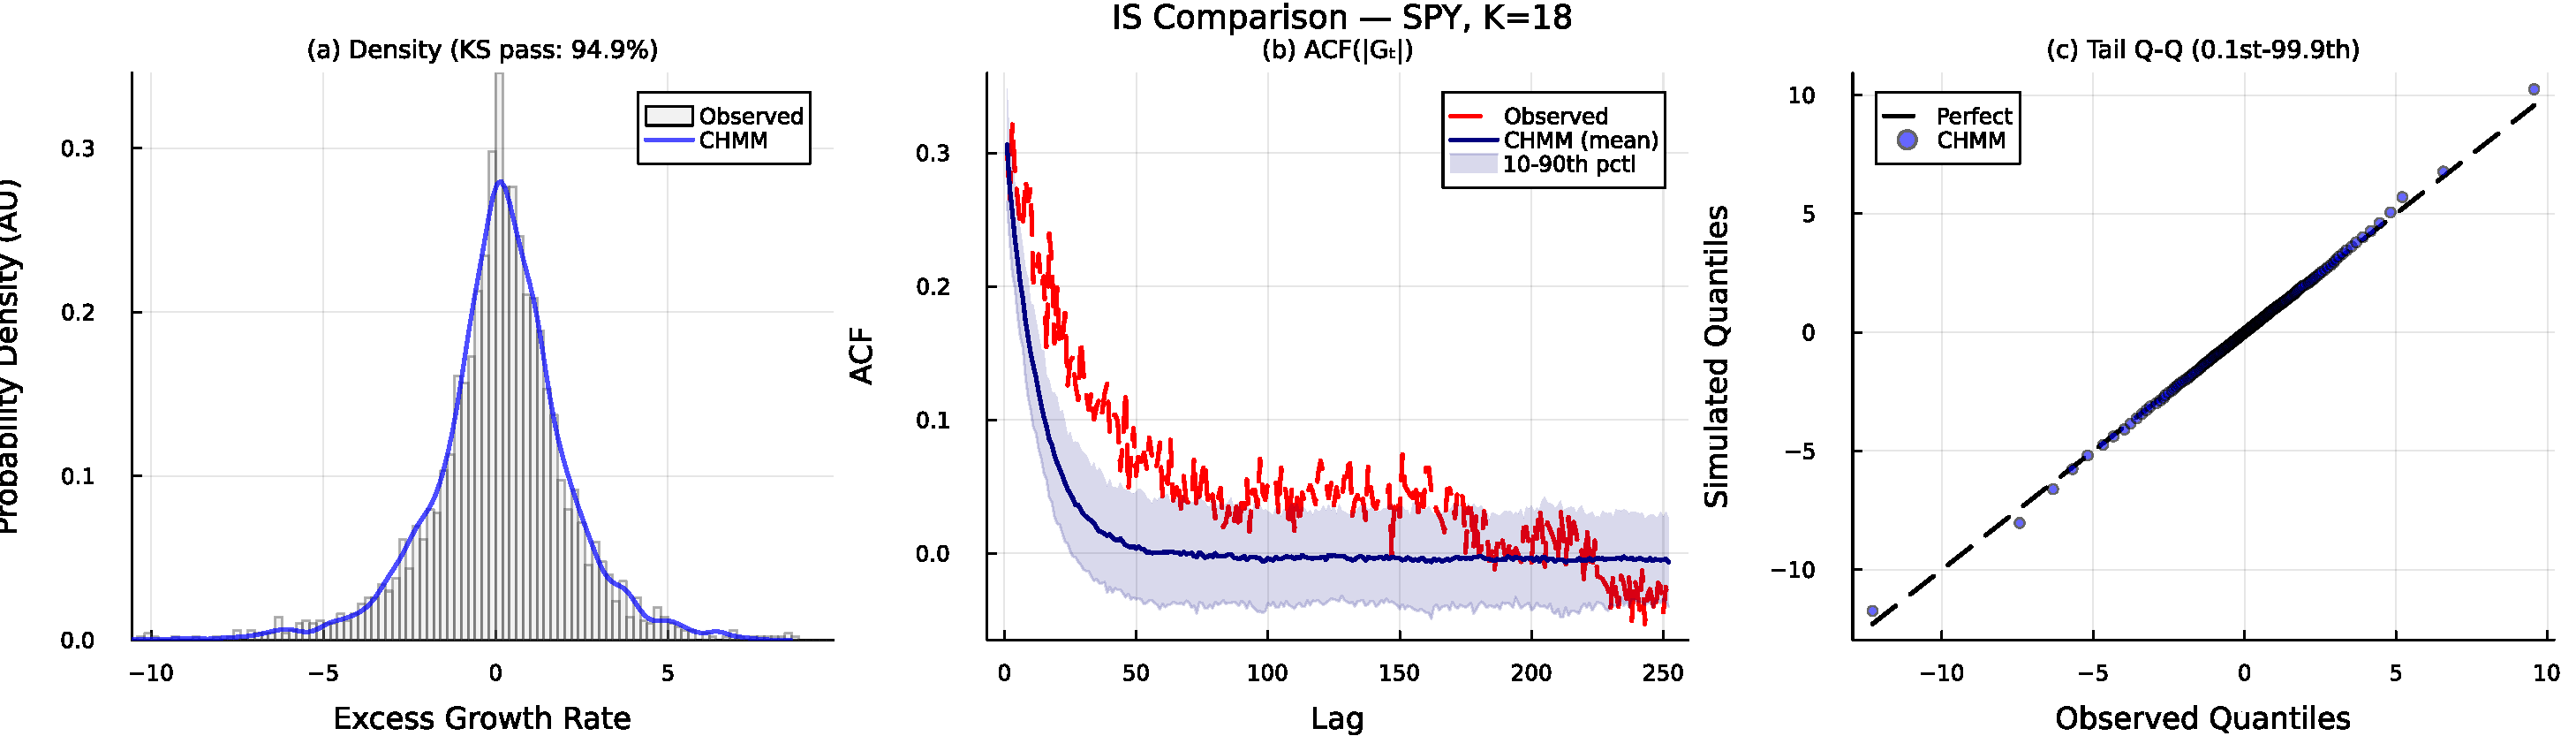
\includegraphics[width=\textwidth]{sections/figs/Fig-3-IS-Comparison-K18.pdf}
\caption{In-sample model comparison for SPY (1{,}000 paths), $K = 18$. (a)~Marginal density with KS pass rates annotated. (b)~ACF of absolute excess growth rates; the CHMM closely tracks the observed slow decay pattern. (c)~Tail Q-Q plot comparing simulated quantiles to observed.}
\label{fig:is_comparison}
\end{figure}

\subsection{State Resolution Sensitivity}
\label{sec:k_sensitivity}

Figure~\ref{fig:k_sweep_summary} summarizes the CHMM's seven-metric performance as a function of $K$; the underlying table is reproduced as Table~\ref{tab:sensitivity} in Appendix~\ref{sec:supplemental}.
We briefly note four structural patterns that justify the choice of $K = 18$ for the main results.

\paragraph{Distributional Fidelity Saturates in the $K \in \{15, 18, 21\}$ Band.}
The IS KS pass rate increased from 88.7\% ($K = 3$) to 95.2\% ($K = 18$) and 96.5\% ($K = 21$); the OoS KS from 92.8\% to 94.0\% at $K = 18$ and 94.9\% at $K = 21$.
The same pattern holds for AD (79.2\% $\to$ 88.3\% IS and 84.9\% $\to$ 88.7\% OoS at $K = 18$).
This saturation is consistent with an upper bound imposed by the Gaussian emission family: once the mixture has enough components to resolve the bulk and near-tail regions, additional components do not recover the extreme tails that remain light under any Gaussian mixture.

\paragraph{Temporal Fidelity Is Flat Across the Sweep.}
ACF-MAE was 0.0453 ($K=3$) to 0.0505 ($K=18$) and 0.0503 ($K=21$) for CHMM-N --- a total swing of 0.005 across the entire sweep.
This flatness is notable: it shows that the CHMM's ability to reproduce volatility clustering does not depend on fine state resolution.
Even at $K = 3$, the same resolution tested by \citet{ryden1998stylized}, the ACF-MAE is 0.0453, comparable to GARCH(1,1) at 0.047.
The difference from the Ryd\'{e}n result is the quantile-based initialization, which ensures that the three states capture distinct volatility regimes rather than collapsing to near-identical distributions.

\paragraph{Kurtosis Is Non-Monotonic and Peaks in the Plateau Band.}
Simulated kurtosis under CHMM-N ranged from 3.70 ($K=9$) to 5.13 ($K=6$), with $K=18$ at 5.03; at higher $K$ the mixture kurtosis oscillates within the 4.5--5.1 band.
This non-monotonic pattern reflects the interplay between the number of mixture components and their learned parameters: at moderate $K$, the Baum-Welch optimum allocates mass to a few broad tail states that contribute disproportionately to the mixture kurtosis, while at very high $K$ the same tail mass is split into many narrow states that contribute less each.
The heavy-tailed CHMM-t and CHMM-L variants close most of this gap at the same $K = 18$ (see Table~\ref{tab:sensitivity_multi}).

\paragraph{Wasserstein, Hellinger, and Coverage Are Monotonic.}
$W_1$ improved monotonically from 0.119 ($K=3$) to 0.101 ($K=18$), Hellinger from 0.079 to 0.077, and Coverage was 100\% at every $K$.
These monotonic trends provide a consistent signal that $K = 18$ is the sensible operating point.

\begin{figure}[t]
\centering
\begin{subfigure}[b]{0.48\textwidth}
    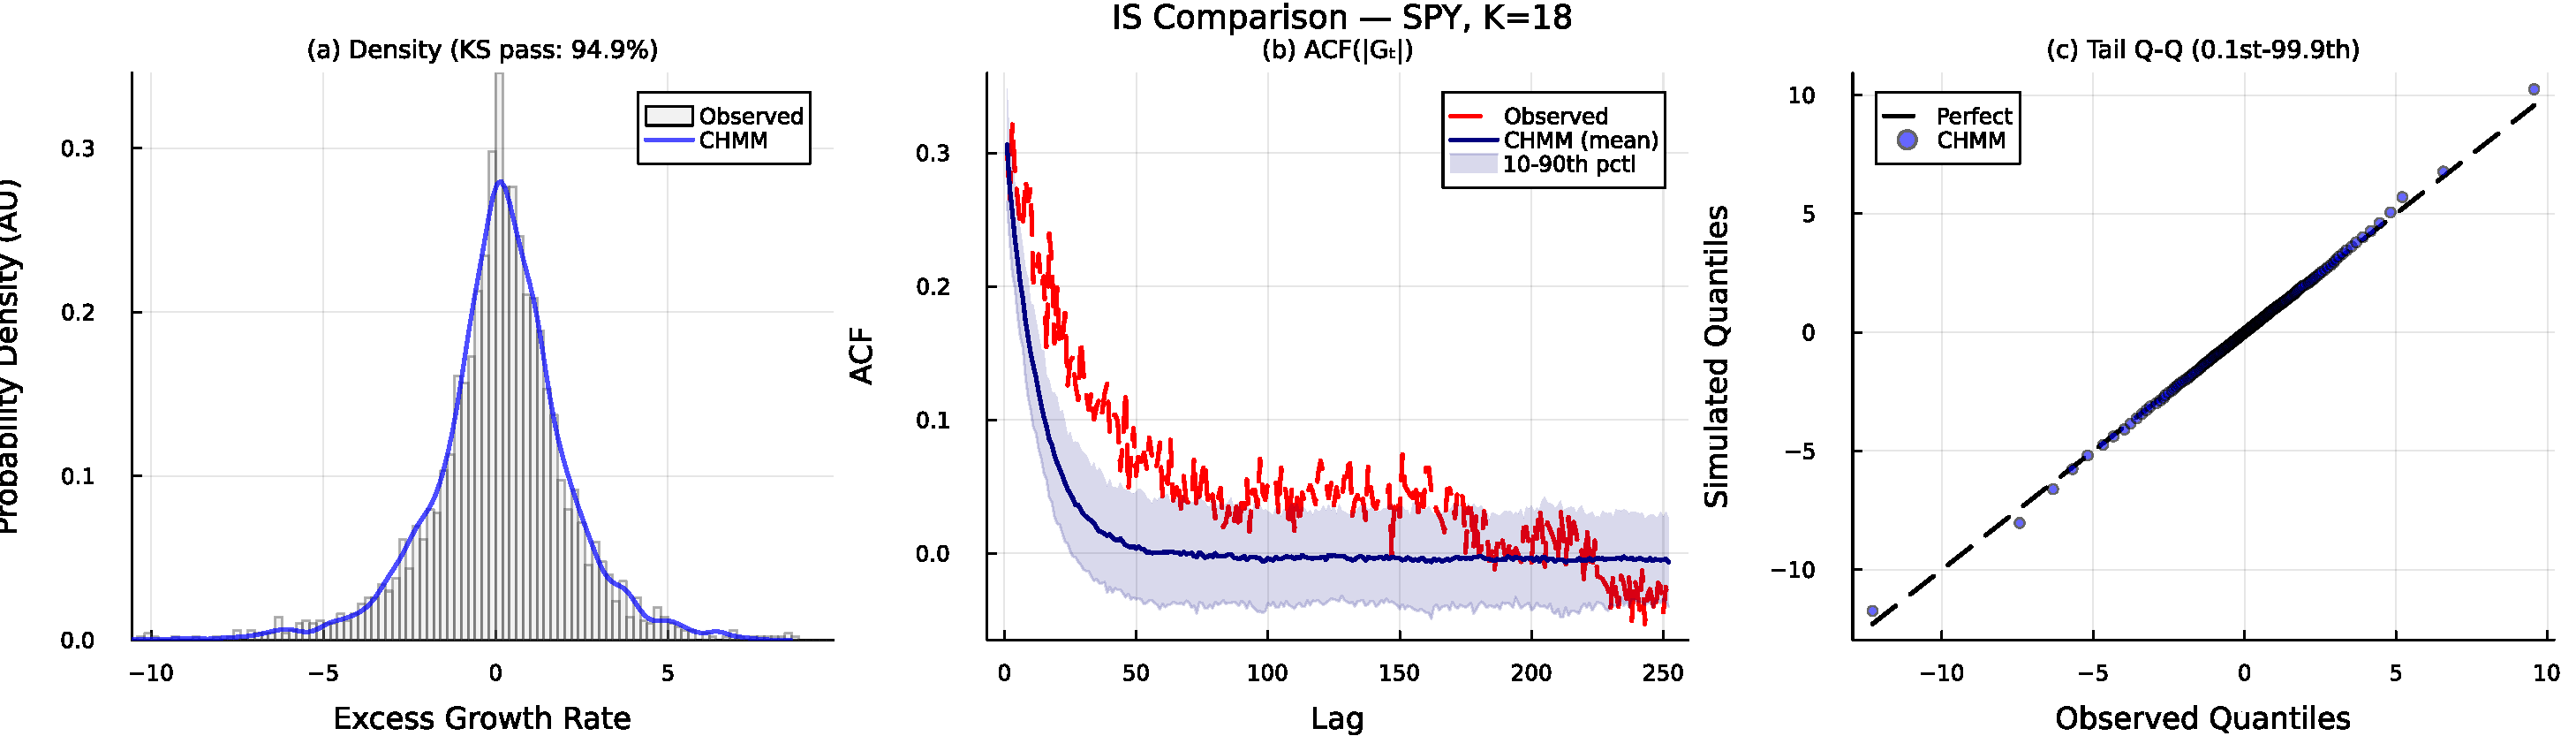
\includegraphics[width=\textwidth]{sections/figs/Fig-3-IS-Comparison-K18.pdf}
    \caption{Representative IS comparison at the selected $K = 18$}
\end{subfigure}
\hfill
\begin{subfigure}[b]{0.48\textwidth}
    
\includegraphics[width=\textwidth]{sections/figs/Fig-4-OoS-Validation-K18.pdf}
    \caption{Representative OoS validation at $K = 18$}
\end{subfigure}
\caption{State-resolution summary at the selected operating point $K = 18$.
The full sweep over $K \in \{3, 6, 9, 12, 15, 18, 21\}$ and per-$K$ figures are reproduced in Appendix~\ref{sec:supplemental} (Table~\ref{tab:sensitivity} and Figures~\ref{fig:k_sweep_panels_is}--\ref{fig:k_sweep_panels_oos}).}
\label{fig:k_sweep_summary}
\end{figure}

\subsection{Out-of-Sample Evaluation}
\label{sec:oos}

At the selected state resolution $K = 18$ the CHMM-N achieves 94.7\% OoS KS pass rate, 88.0\% OoS AD pass rate, and 100\% OoS quantile coverage on the 2025 holdout window; the heavy-tailed CHMM-t and CHMM-L variants reach 95.2\%/90.0\% and 93.9\%/91.7\% OoS KS/AD, respectively.
The CHMM-N OoS simulated kurtosis is 3.45 against an observed 6.24, a shrinkage proportional to the IS gap; CHMM-t closes this to 6.42 and CHMM-L to 5.06.
Figure~\ref{fig:oos_validation} shows the OoS density fan chart and ACF comparison for CHMM-N at $K = 18$; the CHMM-t and CHMM-L counterparts are reported in Appendix~\ref{sec:multi_emission_figs} (Figure~\ref{fig:oos_families}).

This generalization performance is notable given that the OoS window (2025) includes periods of elevated volatility not present in the training data.
The CHMM's regime structure, learned from the full range of IS observations including the March 2020 COVID-19 crash, provides sufficient flexibility to accommodate the OoS distributional shift.

\begin{figure}[t]
\centering

\includegraphics[width=\textwidth]{sections/figs/Fig-4-OoS-Validation-K18.pdf}
\caption{Out-of-sample validation of CHMM ($K = 18$, $\alpha = 0.05$). (a)~KS $p$-values for 1{,}000 OoS paths. (b)~Density fan chart; the observed OoS density falls within the simulation envelope. (c)~OoS ACF of $|G_t|$ with 10th--90th percentile band.}
\label{fig:oos_validation}
\end{figure}

\subsection{Utility: VaR and Expected-Shortfall Back-Test}
\label{sec:utility}

Fidelity (Section~\ref{sec:model_comparison}) measures how close the simulated distribution is to the observed one at the univariate level.
Utility measures whether a downstream consumer of the synthetic paths arrives at the same quantitative conclusion that the historical data would produce.
For a financial-risk consumer the canonical diagnostics are one-tail Value-at-Risk (VaR) and Expected-Shortfall (ES) at daily probability levels of $1\%$ and $5\%$; the synthetic-data generator is well calibrated if the envelope of per-path simulated VaR/ES brackets the observed historical VaR/ES.
We simulate $1{,}000$ independent paths of length $T_{\text{IS}} = 2{,}766$ and $T_{\text{OoS}} = 219$ from each of the five models most relevant to the comparison (Bootstrap, GARCH(1,1), CHMM-N, CHMM-t, CHMM-L) and, on each path, compute the left-tail $1\%$ and $5\%$ VaR and the associated ES.
Table~\ref{tab:var_es} reports the median and $[5\%, 95\%]$ envelope of each quantity across paths alongside the observed historical value.

\begin{table}[t]
\centering
\caption{VaR and Expected-Shortfall back-test calibration for SPY (seed = 20260420, $1{,}000$ paths). Each entry shows the median and $[5\%, 95\%]$ envelope across paths of the left-tail VaR / ES at the stated level. Observed historical values given in the first row. A well-calibrated generator brackets the observed value within its envelope.}
\label{tab:var_es}
\small
\resizebox{\textwidth}{!}{%
\begin{tabular}{l l l l l}
\toprule
          & IS VaR$_{0.01}$              & IS ES$_{0.01}$               & IS VaR$_{0.05}$              & IS ES$_{0.05}$               \\
Model     & median $[5\%, 95\%]$         & median $[5\%, 95\%]$         & median $[5\%, 95\%]$         & median $[5\%, 95\%]$         \\
\midrule
\textit{Observed}  & $-6.36$                      & $-8.83$                      & $-3.36$                      & $-5.36$                      \\
Bootstrap & $-6.36\ [-6.87, -5.86]$      & $-8.70\ [-10.04,\ -7.67]$    & $-3.35\ [-3.60, -3.16]$      & $-5.33\ [-5.79, -4.93]$      \\
GARCH     & $-5.62\ [-7.96, -4.51]$      & $-7.54\ [-12.35,\ -5.67]$    & $-3.14\ [-3.77, -2.73]$      & $-4.74\ [-6.43, -3.89]$      \\
CHMM-N    & $-6.63\ [-7.82, -5.50]$      & $-8.77\ [-9.97,\ -7.48]$     & $-3.32\ [-3.87, -2.91]$      & $-5.34\ [-6.17, -4.56]$      \\
CHMM-t    & $-6.44\ [-7.26, -5.64]$      & $-8.93\ [-10.45,\ -7.67]$    & $-3.32\ [-3.73, -2.88]$      & $-5.36\ [-5.97, -4.74]$      \\
CHMM-L    & $-6.72\ [-7.55, -5.87]$      & $-8.98\ [-10.14,\ -7.90]$    & $-3.24\ [-3.66, -2.81]$      & $-5.40\ [-5.97, -4.76]$      \\
\midrule
          & OoS VaR$_{0.01}$             & OoS ES$_{0.01}$              & OoS VaR$_{0.05}$             & OoS ES$_{0.05}$              \\
\textit{Observed}  & $-6.79$                      & $-9.46$                      & $-3.28$                      & $-5.98$                      \\
Bootstrap & $-6.01\ [-8.58, -4.42]$      & $-7.42\ [-11.56,\ -5.19]$    & $-3.24\ [-4.20, -2.57]$      & $-5.17\ [-6.86, -3.90]$      \\
GARCH     & $-4.63\ [-10.01, -3.07]$     & $-5.38\ [-11.41,\ -3.50]$    & $-3.00\ [-5.65, -2.08]$      & $-4.12\ [-8.42, -2.77]$      \\
CHMM-N    & $-5.73\ [-9.59, -3.23]$      & $-7.17\ [-11.41,\ -3.82]$    & $-3.16\ [-5.49, -2.03]$      & $-4.91\ [-7.88, -2.98]$      \\
CHMM-t    & $-5.86\ [-8.77, -3.40]$      & $-7.45\ [-12.29,\ -4.38]$    & $-3.15\ [-4.67, -2.01]$      & $-5.13\ [-7.45, -3.08]$      \\
CHMM-L    & $-6.05\ [-8.95, -3.35]$      & $-7.48\ [-11.28,\ -4.55]$    & $-3.04\ [-4.60, -2.07]$      & $-5.16\ [-7.15, -3.22]$      \\
\bottomrule
\end{tabular}%
}
\end{table}

Two findings are central to the utility story.
First, all three CHMM variants bracket the observed historical VaR and ES at both $1\%$ and $5\%$ levels within their $5\%$--$95\%$ envelopes on both IS and OoS windows; the in-sample CHMM-L median VaR$_{0.01}$ at $-6.72$ (observed $-6.36$) and the CHMM-N median ES$_{0.01}$ at $-8.77$ (observed $-8.83$) are the closest point estimates across the five generators.
In-sample the three CHMMs are therefore well calibrated as risk consumers and carry narrower uncertainty bands than GARCH (whose $[-7.96, -4.51]$ VaR$_{0.01}$ envelope is roughly $1.7\times$ wider than the CHMMs').
Second, CHMM-t -- despite overshooting the empirical kurtosis by $63\%$ in-sample -- does \emph{not} produce a systematically more conservative VaR/ES estimate: its in-sample median VaR$_{0.01}$ of $-6.44$ is almost identical to CHMM-N's $-6.63$, and its envelope width is comparable.
The CHMM-t kurtosis overshoot therefore translates into a modestly widened uncertainty band rather than a biased point estimate, so a practitioner using CHMM-t for tail-risk scenario generation does not systematically overstate $1\%$ or $5\%$ quantile risk.
Figure~\ref{fig:var_es} visualizes the envelopes alongside the historical observations.

\begin{figure}[t]
\centering
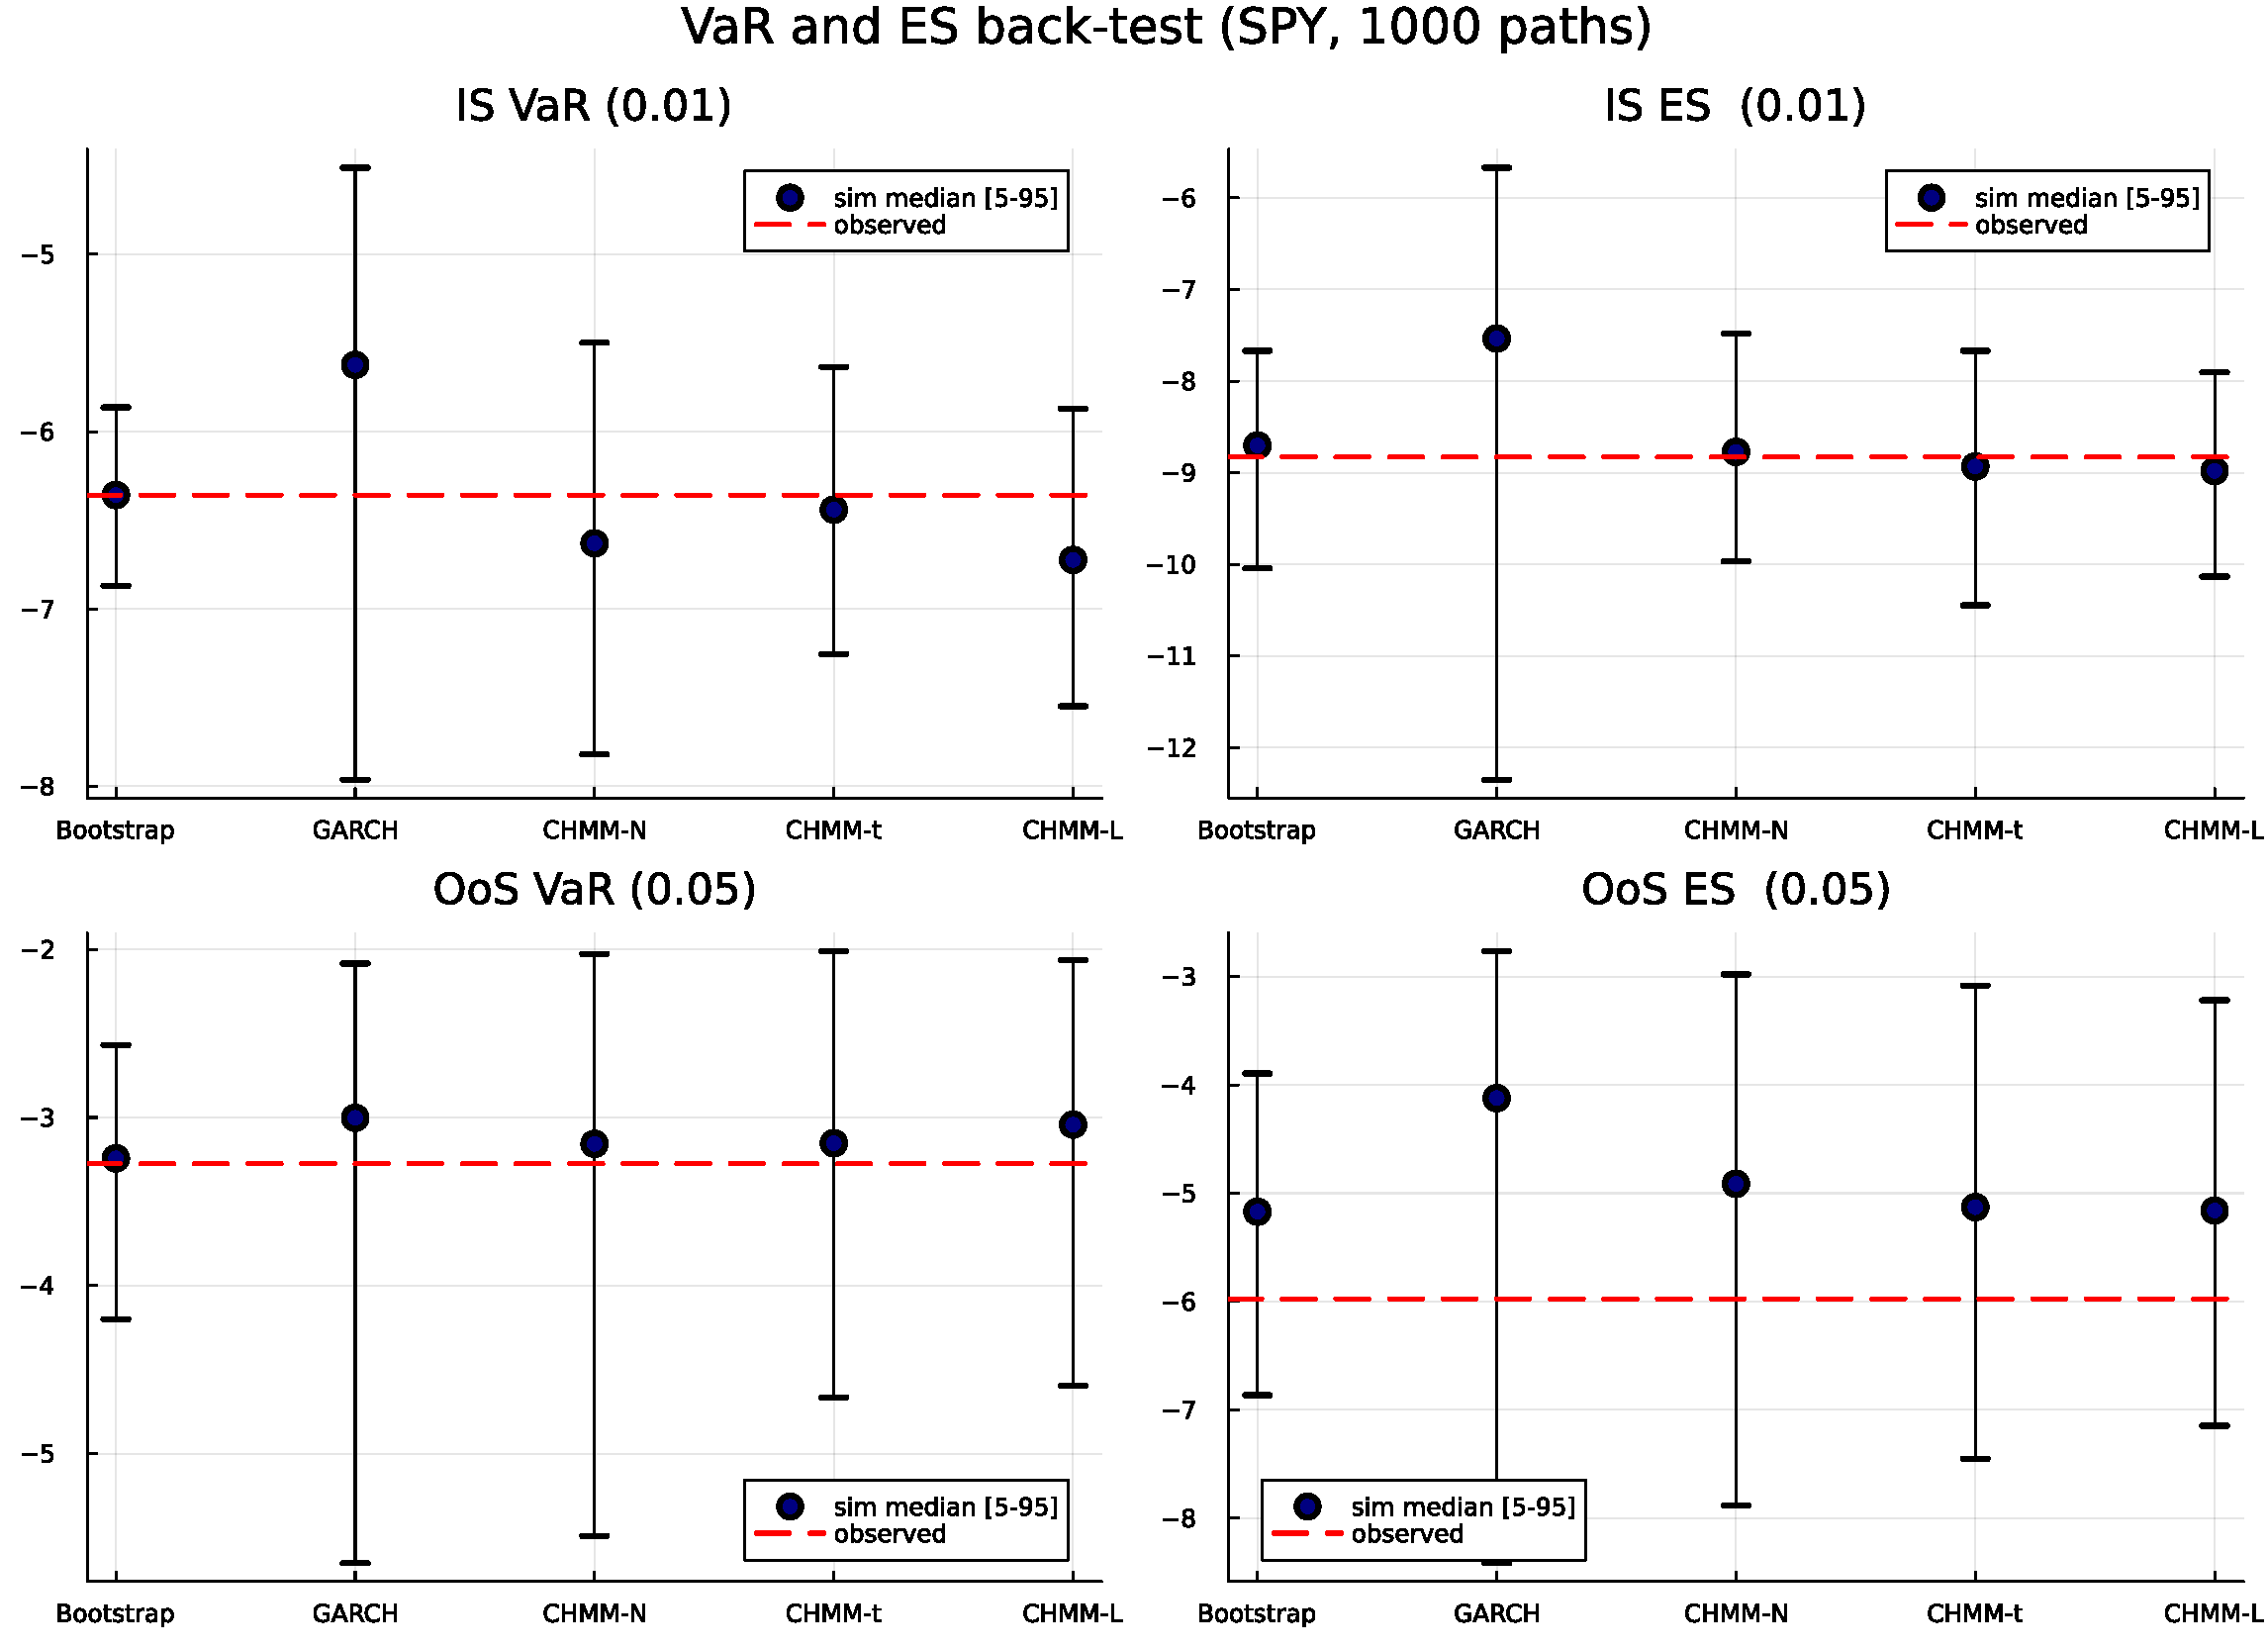
\includegraphics[width=0.98\textwidth]{sections/figs/Fig-v7-VaR-ES.pdf}
\caption{VaR and Expected-Shortfall back-test calibration (SPY, $1{,}000$ simulated paths, seed = 20260420). Each subplot shows the simulated median and $[5\%, 95\%]$ envelope (error bars) across paths and the observed historical value (dashed red line). All three CHMM variants bracket the observed historical VaR and ES at both confidence levels on both in-sample and out-of-sample windows.}
\label{fig:var_es}
\end{figure}

\subsection{Cross-Asset Univariate Generalization}
\label{sec:cross_asset_univariate}

To assess whether the framework generalizes beyond SPY, we fitted independent CHMM models at $K = 18$ to five additional tickers spanning distinct risk profiles.
Table~\ref{tab:cross_asset} reports the results.
Three patterns are worth highlighting.

\paragraph{High-Beta Technology and Broad Market.}
SPY (95.9\% IS / 95.5\% OoS KS), NVDA (99.1\% / 97.5\%), AAPL (99.4\% / 98.6\%), and QQQ (94.5\% / 95.8\%) all show strong IS \emph{and} OoS fidelity under CHMM-N.
The technology-heavy names have lower observed kurtosis (3.3--5.0) than the broader market (SPY: 7.7) and the CHMM tracks them tightly.

\paragraph{Low-Beta Defensives.}
JNJ (99.4\% IS / 68.4\% OoS KS) and JPM (98.0\% IS / 72.0\% OoS KS) show the largest IS-to-OoS degradation in the study, with the OoS drop concentrated in the 2025 holdout window.
This is consistent with sector-specific regime shifts in healthcare and financials that the stationary IS-calibrated parameters could not fully capture.
We return to this finding in Section~\ref{sec:discussion}, where we argue that it is not a consequence of over- or under-fitting $K$ (it reproduces at every $K$ in the sweep), but rather of the stationarity assumption imposed by a single-pass Baum-Welch fit.

\paragraph{Walk-Forward Rolling-Window Re-Estimation on Defensives.}
To test the stationarity explanation directly, we refit the CHMM-N at $K = 18$ quarterly (every $63$ trading days) across the $2025$ OoS window, feeding the realized returns of each completed quarter back into the training set before the next refit (Appendix~\ref{sec:walk_forward}, Table~\ref{tab:walk_forward}).
The rolling-window fit narrows the OoS gap on both tickers: JNJ moves from $70.2\%$ to $71.0\%$ OoS KS and from $61.5\%$ to $62.9\%$ OoS AD, JPM from $74.9\%$ to $76.8\%$ OoS KS and from $76.5\%$ to $78.1\%$ OoS AD, with OoS simulated kurtosis unchanged at the family level.
The modest $\sim 1$--$2$ percentage-point recovery shows that rolling re-estimation is a partial remedy rather than a complete one: sector-specific structural breaks in $2025$ appear to move the defensives' return distribution in ways that a quarterly re-fit, constrained to the same $K$ and emission family, cannot fully absorb.
This supports the stationarity explanation as the principal contributor to the OoS gap while leaving a residual term that a richer extension (time-varying emission scales, or a Bayesian online transition-matrix update) would be needed to close.

\paragraph{Kurtosis: CHMM-L matches observed, CHMM-t overshoots, CHMM-N understates.}
At $K = 18$, the three CHMM variants produce a consistent ordering on the kurtosis diagnostic across the panel (Table~\ref{tab:cross_asset}): CHMM-N simulated kurtosis systematically underestimates observed (observed 3.3--8.6 vs.\ simulated 1.9--7.9); CHMM-L produces values clustered closely around observed (3.49--6.58) and is closest to observed on five of six assets; CHMM-t overshoots on several tickers (e.g.\ 78.0 for JNJ, 53.3 for NVDA), reflecting states that find very small $\nu_k$ inside the ECM search on thin-tailed assets.
Despite this spread in simulated kurtosis, all three variants achieve IS KS pass rates above 93.5\% and IS AD above 87.5\% on every asset, confirming that the mixture can accommodate a wide range of tail weights without sacrificing central fit.

\begin{table}[t]
\centering
\caption{Cross-asset univariate generalization across the three CHMM emission variants ($K = 18$, 1{,}000 paths, $\alpha = 0.05$). Each ticker fitted independently.
CHMM-N, CHMM-t, CHMM-L denote Gaussian, Student-t, and Laplace emissions respectively.}
\label{tab:cross_asset}
\resizebox{\textwidth}{!}{%
\small
\begin{tabular}{l l cc c cc c c c c}
\toprule
& & \multicolumn{2}{c}{KS (\%)} & AD IS (\%) & \multicolumn{2}{c}{Kurtosis} & & & & \\
\cmidrule(lr){3-4} \cmidrule(lr){6-7}
Ticker & Variant & IS & OoS & & Obs & Sim & ACF-MAE & $W_1$ & $H$ & Cov IS (\%) \\
\midrule
SPY  & CHMM-N & 95.9 & 95.5 & 90.5 & 7.7 & 5.05  & 0.0503 & 0.101 & 0.0768 & 100.0 \\
     & CHMM-t & 96.2 & 95.0 & 91.4 & 7.7 & 15.81 & 0.0539 & 0.093 & 0.0719 & 100.0 \\
     & CHMM-L & 93.7 & 92.8 & 91.0 & 7.7 & 6.42  & 0.0544 & 0.095 & 0.0756 & 100.0 \\
\midrule
NVDA & CHMM-N & 99.1 & 97.5 & 97.7 & 5.0 & 3.28  & 0.0420 & 0.232 & 0.0865 & 99.0  \\
     & CHMM-t & 99.4 & 98.9 & 98.8 & 5.0 & 53.28 & 0.0444 & 0.221 & 0.0742 & 100.0 \\
     & CHMM-L & 99.3 & 99.0 & 98.4 & 5.0 & 3.49  & 0.0443 & 0.209 & 0.0836 & 100.0 \\
\midrule
JNJ  & CHMM-N & 99.4 & 68.4 & 99.0 & 8.6 & 5.71  & 0.0319 & 0.084 & 0.0755 & 100.0 \\
     & CHMM-t & 100.0 & 68.1 & 99.6 & 8.6 & 78.00 & 0.0319 & 0.091 & 0.0708 & 100.0 \\
     & CHMM-L & 99.1 & 67.9 & 98.4 & 8.6 & 6.10  & 0.0319 & 0.083 & 0.0758 & 100.0 \\
\midrule
JPM  & CHMM-N & 98.0 & 72.0 & 94.9 & 8.0 & 7.94  & 0.0434 & 0.151 & 0.0837 & 100.0 \\
     & CHMM-t & 98.2 & 76.6 & 96.6 & 8.0 & 14.24 & 0.0439 & 0.144 & 0.0800 & 100.0 \\
     & CHMM-L & 100.0 & 83.0 & 99.2 & 8.0 & 6.58  & 0.0466 & 0.132 & 0.0819 & 100.0 \\
\midrule
AAPL & CHMM-N & 99.4 & 98.6 & 98.6 & 3.3 & 2.48  & 0.0402 & 0.134 & 0.0842 & 100.0 \\
     & CHMM-t & 98.9 & 98.5 & 97.8 & 3.3 & 7.55  & 0.0406 & 0.126 & 0.0807 & 100.0 \\
     & CHMM-L & 98.6 & 97.6 & 97.4 & 3.3 & 4.01  & 0.0409 & 0.128 & 0.0845 & 100.0 \\
\midrule
QQQ  & CHMM-N & 94.5 & 95.8 & 87.7 & 3.3 & 1.91  & 0.0524 & 0.119 & 0.0700 & 100.0 \\
     & CHMM-t & 95.8 & 95.3 & 92.2 & 3.3 & 3.18  & 0.0536 & 0.109 & 0.0714 & 100.0 \\
     & CHMM-L & 93.7 & 95.3 & 93.4 & 3.3 & 4.94  & 0.0562 & 0.121 & 0.0768 & 100.0 \\
\bottomrule
\end{tabular}%
}
\end{table}

\subsection{Cross-Asset Dependence: SIM and Copula Extensions}
\label{sec:cross_asset}

Section~\ref{sec:cross_asset_univariate} established that the CHMM provides strong per-asset univariate fidelity across distinct risk profiles.
The next question is whether we can assemble those univariate marginals into jointly plausible multi-asset paths.
We instantiated the two constructions described in Section~\ref{sec:cross_asset_methods} on a six-asset universe (SPY, NVDA, JNJ, JPM, AAPL, QQQ) with SPY as the market engine, using the common in-sample window (2014--2024, $T = 2{,}766$) and CHMM marginals refitted at $K = 18$.
Table~\ref{tab:cross_asset_sim_copula} reports the per-asset KS pass rates and cross-sectional correlation reproduction across 200 simulated paths.

\paragraph{SIM (Single Index Model).}
The ordinary least squares regression of each asset against SPY produced a range of factor loadings (high $\beta$ for NVDA, $\hat{\beta} = 1.75$; low $\beta$ for JNJ, $\hat{\beta} = 0.54$) and goodness-of-fit $R^2$ from 0.225 (JNJ) to 0.841 (QQQ).
When propagated through the factor equation~\eqref{eq:sim_sim}, the SIM produced uneven per-asset distributional fidelity.
The market-factor asset SPY preserved 94.0\% IS KS by construction.
Non-market assets' IS KS pass rates fell across a wide range: 92.0\% (JNJ), 85.5\% (QQQ), 82.0\% (AAPL), 81.0\% (NVDA), and 36.0\% (JPM).
The severe JPM degradation (36.0\% IS KS) reflects the fact that the affine map $\alpha + \beta G_M$ applied to a Gaussian-mixture market factor does not preserve JPM's empirical tail structure once residuals are re-injected: the residual distribution is centered but heavy-tailed enough to violate JPM's own marginal at the 5\% KS threshold.
Cross-sectional correlation reproduction was acceptable on average (off-diagonal MAE 0.078) but visibly worse than both copulas, consistent with SIM's rank-one decomposition discarding joint information beyond the market factor.

\paragraph{Gaussian copula.}
The Gaussian copula achieved a median per-asset in-sample KS pass rate of 97.8\%, with every asset above 93\% (the minimum was 93.5\% for QQQ).
This uniform distributional fidelity is the expected consequence of rank reordering: each column of the simulated matrix is a permutation of an independent CHMM path, so the marginal distribution is preserved exactly.
The off-diagonal correlation MAE of 0.031 improved by a factor of 2.5 over the SIM baseline.

\paragraph{Student-t copula.}
Profile maximum likelihood over $\nu \in \{2, 3, 4, 5, 6, 8, 10, 15, 20, 30\}$ selected $\nu^* = 6$, indicating non-trivial joint tail dependence.
The Student-t copula matched the Gaussian copula's median IS KS pass rate (99.0\% vs.\ 97.8\%) and nudged ahead on the mean (98.2\% vs.\ 97.5\%).
It also achieved the best correlation reproduction overall, with off-diagonal MAE of 0.027 and Frobenius norm of 0.181 (versus 0.031 and 0.203 for the Gaussian copula).
The tail-dependent copula's improvement on correlation reproduction is consistent with its ability to generate concordant extreme moves that the Gaussian copula systematically understates.

\paragraph{Out-of-sample.}
All three dependence models degraded on the shorter OoS window, but the ordering was preserved (Table~\ref{tab:cross_asset_sim_copula}).
The Student-t copula achieved 93.2\% median OoS KS (Gaussian copula 96.0\%, SIM 93.0\%), and continued to lead on correlation reproduction (off-diagonal MAE 0.213 vs.\ 0.212 Gaussian vs.\ 0.233 SIM).
The larger OoS Frobenius norms reflect sampling variation in the observed OoS correlation matrix on only $T = 219$ days, not a failure of the fitted copula.

\begin{table}[t]
\centering
\caption{Cross-asset dependence models: per-asset KS pass rates (\%) and cross-sectional correlation reproduction. 200 simulated paths. Each asset's marginal is a fitted CHMM ($K = 18$). Market factor: SPY. Student-t copula degrees of freedom selected by profile MLE, $\nu^* = 6$. Correlation distance is $\|\hat{\Sigma}_{\text{sim}} - \hat{\Sigma}_{\text{obs}}\|_F$ (Frobenius) and off-diagonal MAE, each averaged over paths.}
\label{tab:cross_asset_sim_copula}
\small
\begin{tabular}{l cc cc cc}
\toprule
& \multicolumn{2}{c}{SIM} & \multicolumn{2}{c}{Gaussian copula} & \multicolumn{2}{c}{Student-t copula ($\nu^* = 6$)} \\
\cmidrule(lr){2-3} \cmidrule(lr){4-5} \cmidrule(lr){6-7}
Ticker & IS & OoS & IS & OoS & IS & OoS \\
\midrule
SPY   & 94.0 & 91.5 & 97.0 & 94.5 & 95.5  & 93.0 \\
NVDA  & 81.0 & 99.5 & 97.0 & 98.0 & 99.5  & 94.0 \\
JNJ   & 92.0 & 78.5 & 99.5 & 70.5 & 99.5  & 65.5 \\
JPM   & 36.0 & 53.5 & 99.5 & 76.5 & 99.5  & 72.5 \\
AAPL  & 82.0 & 95.5 & 98.5 & 97.5 & 98.5  & 96.0 \\
QQQ   & 85.5 & 94.5 & 93.5 & 97.5 & 97.0  & 93.5 \\
\midrule
Mean   & 78.4 & 85.5 & 97.5 & 89.1 & 98.2 & 85.8 \\
Median & 83.8 & 93.0 & 97.8 & 96.0 & 99.0 & 93.2 \\
\midrule
\multicolumn{7}{l}{\textit{Correlation reproduction (averaged over 200 paths)}} \\
Frobenius IS         & \multicolumn{2}{c}{0.542} & \multicolumn{2}{c}{0.203} & \multicolumn{2}{c}{\textbf{0.181}} \\
Off-diag MAE IS      & \multicolumn{2}{c}{0.078} & \multicolumn{2}{c}{0.031} & \multicolumn{2}{c}{\textbf{0.027}} \\
Frobenius OoS        & \multicolumn{2}{c}{1.692} & \multicolumn{2}{c}{\textbf{1.421}} & \multicolumn{2}{c}{1.440} \\
Off-diag MAE OoS     & \multicolumn{2}{c}{0.233} & \multicolumn{2}{c}{\textbf{0.212}} & \multicolumn{2}{c}{0.213} \\
\bottomrule
\end{tabular}
\end{table}

Figure~\ref{fig:cross_asset_corr} visualizes the observed and path-averaged simulated correlation matrices for the three dependence models, and Figure~\ref{fig:cross_asset_ks} shows the per-asset in-sample KS pass rates as a grouped bar chart.
The visual ordering confirms the quantitative summary in Table~\ref{tab:cross_asset_sim_copula}: the SIM introduces visible distortion on JPM and AAPL marginals, while both copulas track the observed marginals closely; on correlation, the SIM panel shows larger residuals off the diagonal than either copula panel, and the Student-t copula is marginally closer to the observed heat map than the Gaussian copula.

\begin{figure}[t]
\centering

\includegraphics[width=0.85\textwidth]{sections/figs/Fig-Cross-Asset-Correlation.pdf}
\caption{In-sample correlation matrix reproduction across dependence models. Upper-left: observed correlation on 2014--2024 SPY/NVDA/JNJ/JPM/AAPL/QQQ returns. Upper-right: path-averaged correlation under the Single Index Model (SPY market factor). Lower-left: path-averaged correlation under the Gaussian copula. Lower-right: path-averaged correlation under the Student-t copula ($\nu^* = 6$). Each simulated panel averages over 200 paths of length $T = 2{,}766$. Per-asset CHMM marginals fitted at $K = 18$.}
\label{fig:cross_asset_corr}
\end{figure}

\begin{figure}[t]
\centering
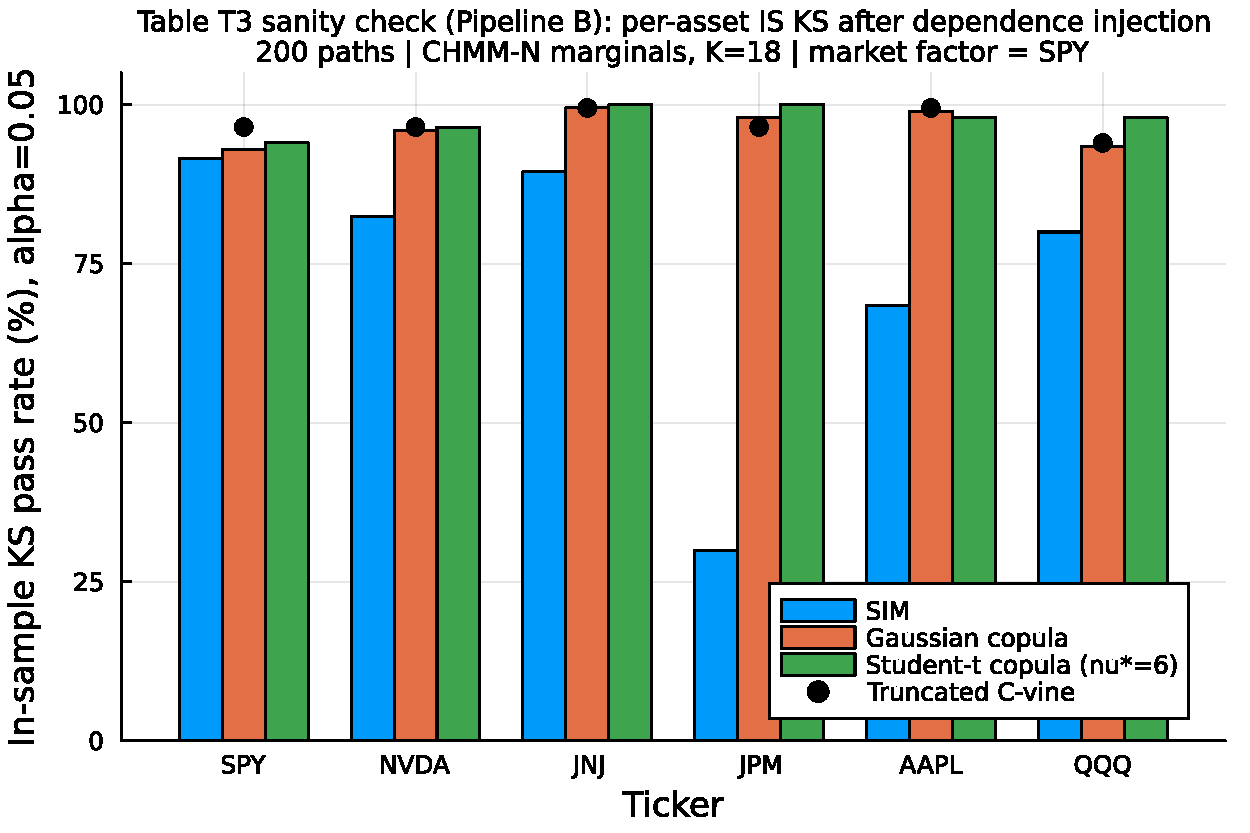
\includegraphics[width=0.85\textwidth]{sections/figs/Fig-Cross-Asset-KS-Dist.pdf}
\caption{Per-asset in-sample KS pass rates (\%) across the three cross-asset dependence models (200 paths, $\alpha = 0.05$). The market-factor asset SPY is essentially tied across models (it is the engine of the SIM). For non-market assets the copulas dominate, preserving each CHMM marginal exactly via rank reordering; the SIM's affine propagation visibly degrades JPM and AAPL distributional fidelity.}
\label{fig:cross_asset_ks}
\end{figure}

\paragraph{Interpretation.}
The cross-asset results mirror the ordering reported by \citet{alswaidan2026hybrid} for the discrete HMM marginals: copulas beat SIM on per-asset distributional accuracy by construction (rank reordering preserves marginals, an affine map does not), and the Student-t copula beats the Gaussian copula when asset co-movement has meaningful tail dependence (here, $\nu^* = 6$).
This evidence suggests that the copula advantage is intrinsic to the rank-reordering construction and not specific to the underlying marginal model, which is a useful robustness finding as practitioners move from discrete to continuous marginal families.

\subsection{Synthetic-Data Generation for VIX}
\label{sec:vix_results}

To test whether the CHMM framework generalizes beyond equity returns we apply it to the CBOE Volatility Index (VIX) daily log-return series.
VIX returns exhibit statistical properties that differ fundamentally from equity excess growth rates: positive skewness (volatility spikes are asymmetric), pronounced mean reversion (crises are transient), and heavier tails.
We fit all three CHMM emission families at $K = 18$ under the same Baum-Welch pipeline, simulate $1{,}000$ paths of length $T_{\text{IS}} = 4{,}713$ and $T_{\text{OoS}} = 317$, and evaluate the same seven-metric battery used in Section~\ref{sec:model_comparison}.
Table~\ref{tab:vix_metrics} reports the full panel.

\begin{table}[t]
\centering
\caption{Three-family CHMM seven-metric panel for VIX (daily log returns, $K = 18$, $1{,}000$ paths, seed = 20260420). Observed IS excess kurtosis $6.56$; OoS $4.05$.}
\label{tab:vix_metrics}
\small
\begin{tabular}{l cc cc cc c c c c}
\toprule
Family & KS IS & AD IS & KS OoS & AD OoS & Kurt IS & Kurt OoS & ACF-MAE & $W_1$ & $H$ & Cov \\
\midrule
CHMM-N & 99.5 & 99.2 & 99.0 & 93.7 & 4.03  & 3.56 & 0.0180 & 0.549 & 0.0667 & 99.0  \\
CHMM-t & 99.4 & 98.8 & 99.2 & 94.8 & 12.59 & 6.41 & 0.0181 & 0.581 & 0.0629 & 100.0 \\
CHMM-L & 99.2 & 98.3 & 98.9 & 93.8 & 5.42  & 4.57 & 0.0179 & 0.582 & 0.0667 & 100.0 \\
\bottomrule
\end{tabular}
\end{table}

All three families achieve strikingly tight distributional and temporal fidelity on VIX: IS KS pass rates of $99.2$--$99.5\%$ and AD of $98.3$--$99.2\%$, with OoS KS of $98.9$--$99.2\%$.
ACF-MAE on $|R_t|$ is $0.018$ -- about three times tighter than the SPY figure -- because VIX's pronounced mean-reversion is a stronger clustering signal than equity volatility clustering.
The three families reproduce the kurtosis differently: CHMM-L sits closest to the observed IS kurtosis of $6.56$ (simulated $5.42$), CHMM-N undershoots ($4.03$) as with equity, and CHMM-t overshoots ($12.59$) in the same direction it overshoots on SPY, confirming that the Student-t overshoot is a property of the emission family rather than of the asset class.
The decoded regime sequence under CHMM-N aligns with known market-stress events, assigning high-volatility states to the 2008 financial-crisis aftermath, the 2011 European debt crisis, the 2015 China devaluation, the 2018 volatility spike, and the March 2020 COVID-19 crash.

\paragraph{Unified Synthetic-Data Engine.}
The VIX and SPY pipelines share identical code, hyperparameters ($K = 18$), and evaluation battery; only the input series changes.
This matches the scope of our prior discrete-HMM paper~\citep{alswaidan2026hybrid}, which also treated VIX as a synthetic-data target on equal footing with equity returns.
Extensions to related volatility measures (VXX futures, VVIX, or foreign-market volatility indices) are immediate under the same pipeline and are outside the scope of this paper.
A detailed breakdown of the VIX CHMM results (convergence, emission PDFs, IS/OoS density panels) is in Appendix~\ref{sec:supplemental}.
